\documentclass[../../topologia_algebraica]{subfiles}
\begin{document}
\section{Cubrientes}

Para calcular grupos de homotop\'ias, es muy \'util la idea de cubrientes. Empiezo con
un ejemplo:

Considera el mapeo exponencial $\epsilon:\RR\ra\Sn^1$, que hace
$t\mapsto e^{2\pi i t}=(\cos 2\pi i t,\sin2\pi i)$ (estoy identificando $\Sn^1\subset\CC$ con
$\Sn^1\subset\RR^2$).
Como $\RR$ se puede encajar en $\RR^3$ como $\imath(t)=(\cos 2\pi i t,\sin2\pi i t,t)$
entonces el mapeo exponencial $\epsilon$ lo puedo pensar como la composici\'on del encaje $\imath$
seguida de la restricci\'on de la proyecci\'on $p:(x_1,x_2,x_3)\mapsto (x_1,x_2)$ en $\RR^3$ porque:
\[
  (p\circ\imath)(t)=
  p(\imath(t))=
  p(\cos 2\pi t,\sin2\pi t,t)=
  (\cos 2\pi t,\sin2\pi t)\in\Sn^1\subset\RR^2 \qquad\quad
  \therefore \epsilon = p\circ\imath.
\]
El siguiente dibujo ilustra esta construcci\'on:
\begin{figure}[ht] %%%%%%%%%%%%%%%%%%%%%%%%%%%%%%%%%%%%%%%%%%%%%%%%%%%%% EXPONENCIAL_CUBRIENTE
  \centering
  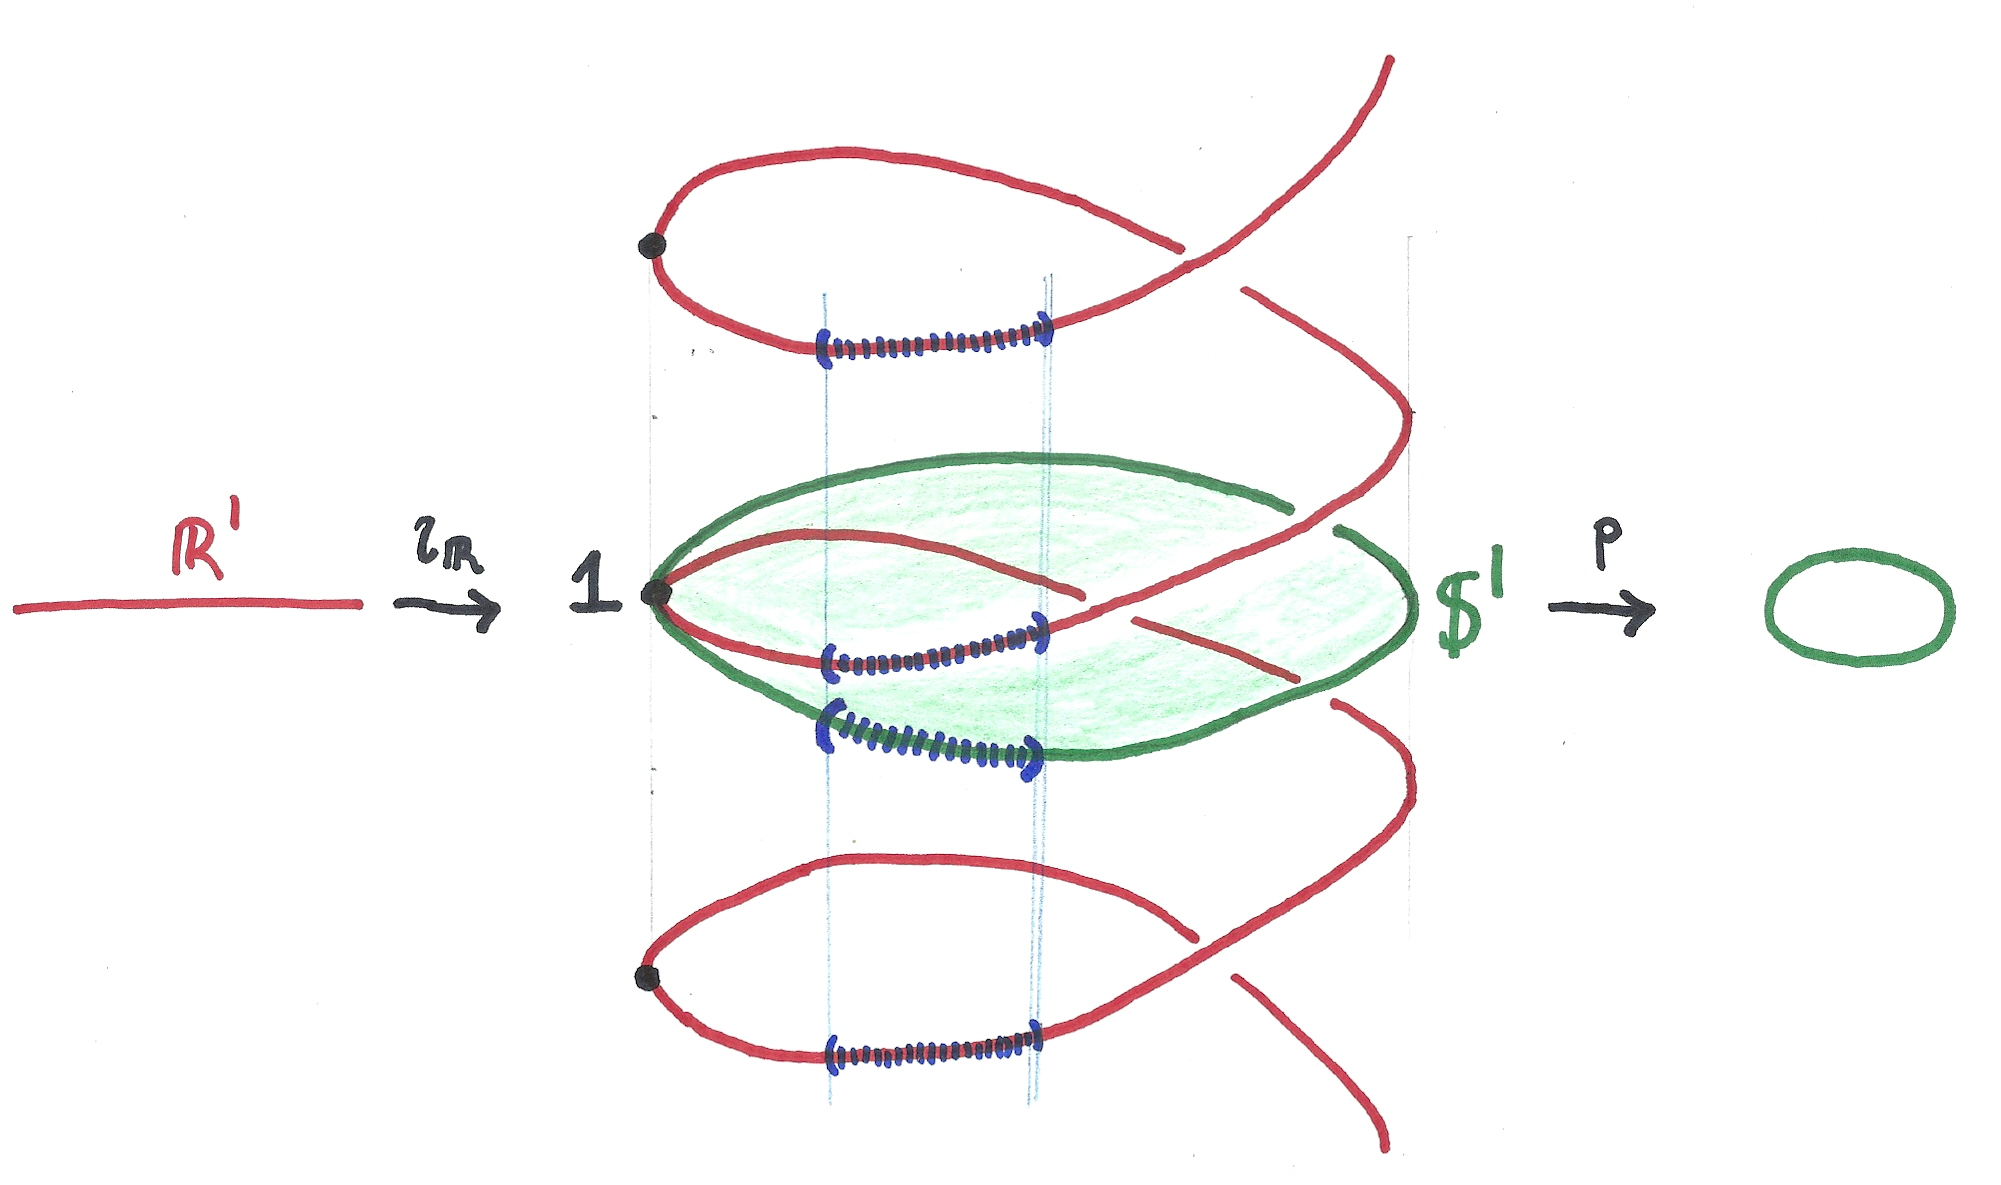
\includegraphics[scale=0.12]{exponencial_cubriente}
\end{figure} %%%%%%%%%%%%%%%%%%%%%%%%%%%%%%%%%%%%%%%%%%%%%%%%%%%%%%%%%%%%%%%%%%%%%%%%%%%%%%%%%%


Para resumir: encajo $\imath:\RR\hookrightarrow\RR^3$ y $\jmath:\Sn^1\hookrightarrow\RR^3$
mediante:
\[
  \imath(t)=(\cos 2\pi t,\sin2\pi t,t) \quad\text{y}\quad
  \jmath(e^{i\theta})=(\cos\theta,\sin\theta,0).
\]
Identifico $\RR=\imath[\RR]$ y $\Sn^1=\jmath[\Sn^1]$. Si $\bar{p}=p|_{\RR}:\RR\ra\Sn^1$ es
la restricci\'on de la proyecci\'on $p:(x_1,x_2,x_3)\mapsto (x_1,x_2)$ en $\RR^3$, entonces
claramente $\epsilon=\bar{p}$.

Esta funci\'on cumple una propiedad muy importante:

\import{\directory}{ejercicios/26} %%%%%%%%%%%%%%%%%%%%%%%%%%%%%%%%%%%%%%%%%%%%%%%%%  EJERCICIO 26

Defino expl\'icitamente esta propiedad:

\begin{defin}
  Sean $E$ y $X$ espacios topol\'ogicos y $p:E\ra X$ una funci\'on continua. La terna $(E,p,X)$
  es un \emph{cubriente} si toda $x\in X$ tiene una vecindad abierta $V\subseteq X$ tal que su
  preimagen es una uni\'on disjunta de abiertos de $E$, ie. $p^{-1}[V]=\bigsqcup U_j$, tal que
  la restricci\'on $p|_{U_j}:U_j\ra V$ es un homeomorfismo.
\end{defin}

\begin{figure}[ht]%%%%%%%%%%%%%%%%%%%%%%%%%%%%%%%%%%%%%%%%%%%%%%%%%%%%%%%%%%%%% FIGURA CUBRIENTES
  \centering
  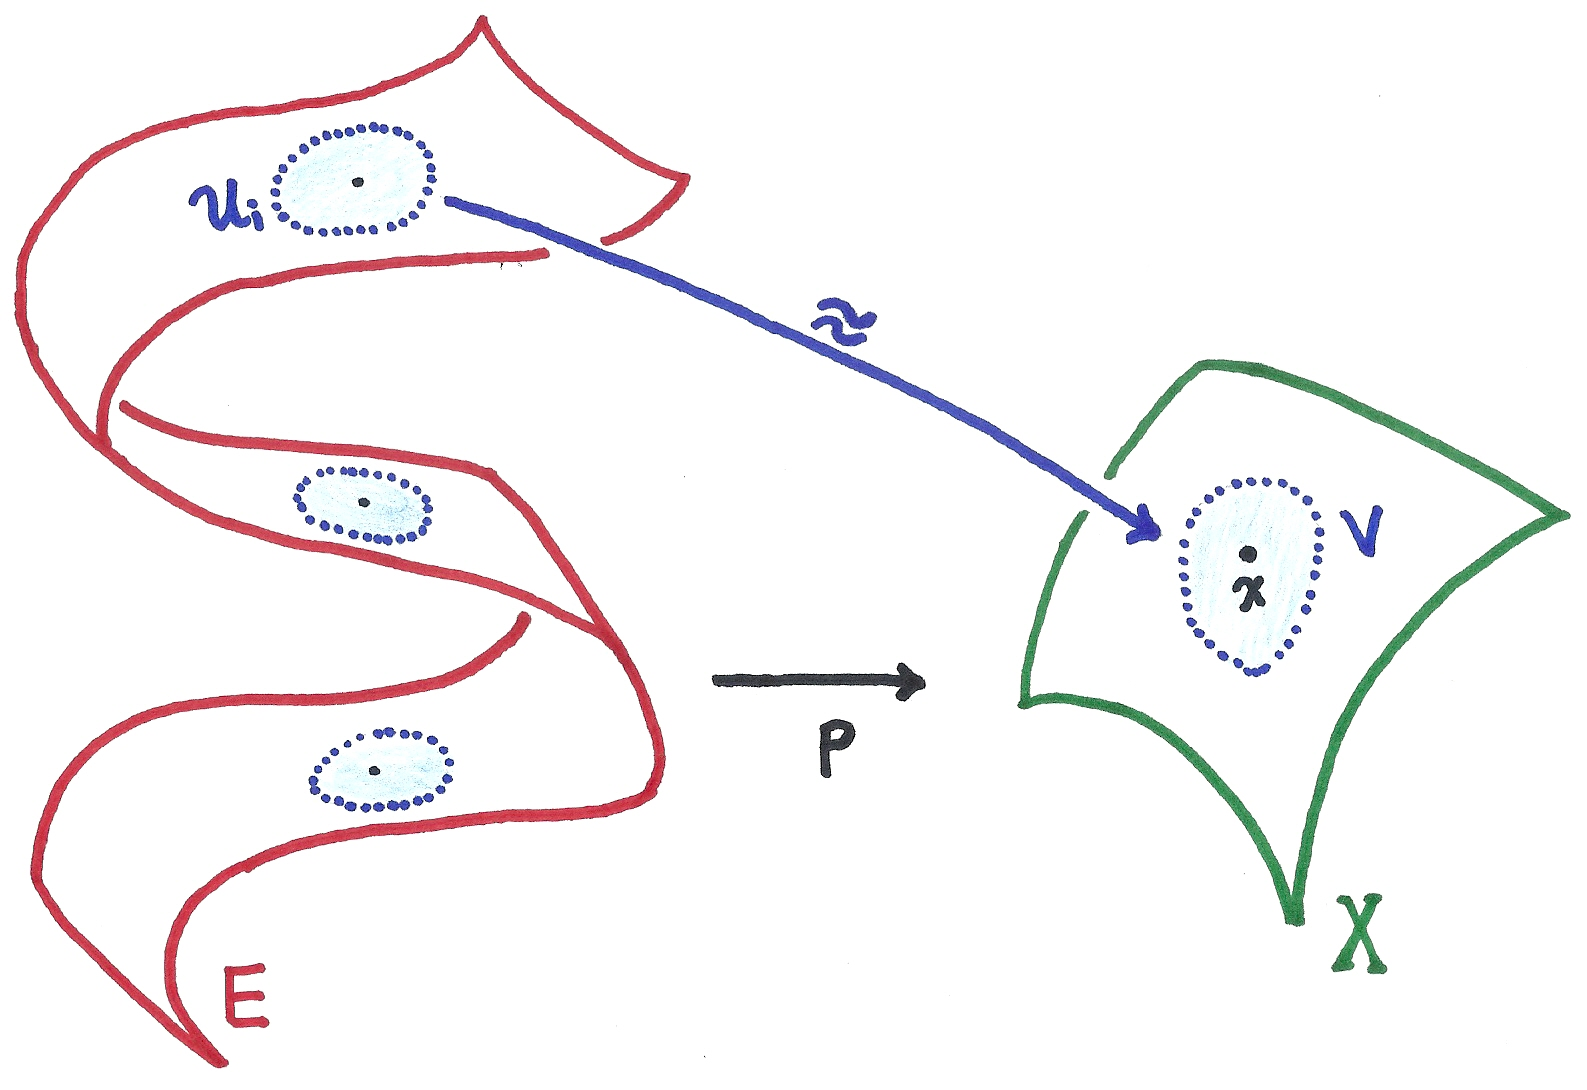
\includegraphics[scale=0.13]{cubriente}
\end{figure}%%%%%%%%%%%%%%%%%%%%%%%%%%%%%%%%%%%%%%%%%%%%%%%%%%%%%%%%%%%%%%%%%%%%%%%%%%%%%%%%%%%%%%


Cada ingrediente de la definici\'on tiene un nombre: $E$ es el \emph{espacio total}, $X$ es el
\emph{espacio base}, la funci\'on $p:E\ra X$ es una \emph{aplicaci\'on cubriente}, las
componentes conexas $U_i$ de $p^{-1}[V]$ se llaman \emph{hojas}. Adem\'as, para un punto
$x\in X$ su imagen inversa $E_x:=p^{-1}[x]$ se llama la \emph{fibra} de $p$ sobre $x$.
A veces dir\'e que la funci\'on $p:E\ra X$ es un cubriente para referirme al cubriente $(E,p,X)$;
esto es porque la notaci\'on de funci\'on ya muestra los tres elementos de la definici\'on de
cubriente.

Las fibras de un cubriente cson discretas:
\begin{prop}
  Sea $p:E\ra X$ un cubriente, $x\in X$ y $E_x\subset E$ la fibra de $p$ sobre $x$. La
  topolog\'ia de $E_x$ como subsespacio de $E$ es la topolog\'ia discreta. 
\end{prop}
\begin{proof}
  Sea $V\subset X$ una vecindad de $x$ tal que $p^{-1}[V]=\bigsqcup U_j$ con $p|_{U_j}$
  es un homeomorfismo sobre su imagen. Ahora, si $e\in E_x$ entonces est\'a en un
  \'unico $U_j$. Por lo tanto si $e'\in E_x\cap U_j$ entonces $p(e)=p(e')$, pero
  $p|_{U_j}$ es inyectivo entonces $e=e'$. Con esto concluyo que los singuletes
  $\{e\}=E_x\cap U_j$ son abiertos y que $E_x$ es un espacio discreto.
\end{proof}

\begin{ejemplo}
  Todo homeomorfismo es un cubriente. Por el ejercicio \ref{ej:26}, la exponencial
  $\epsilon:\RR\ra\Sn^1$ es un cubriente.
\end{ejemplo}

Cubrientes cumplen una propiedad fundamental para el estudio de grupos de homotop\'ias:

\begin{thm}\label{thm:levantamiento}(Levantamiento de trayectorias)
  Sea $p:E\ra X$ un cubriente y $\sigma:I\ra X$ una trayectoria que empieza en $x=\sigma(0)$.
  Para toda $e\in E_{x}$ existe una \'unica trayectoria $\what{\sigma}_e:I\ra E$ que extiende
  a $\sigma$, es decir $p\circ\what{\sigma}_e=\sigma$.
\end{thm}
 %%%%%%%%%%%%%%%%%%%%%%%%%%%%%%%%%%%%%%%%%%%%%%%%%%%%%%%%%%%%%%%%%%%%%%%%%% LEVANTAMIENTO
\begin{figure}[ht]
  \centering
    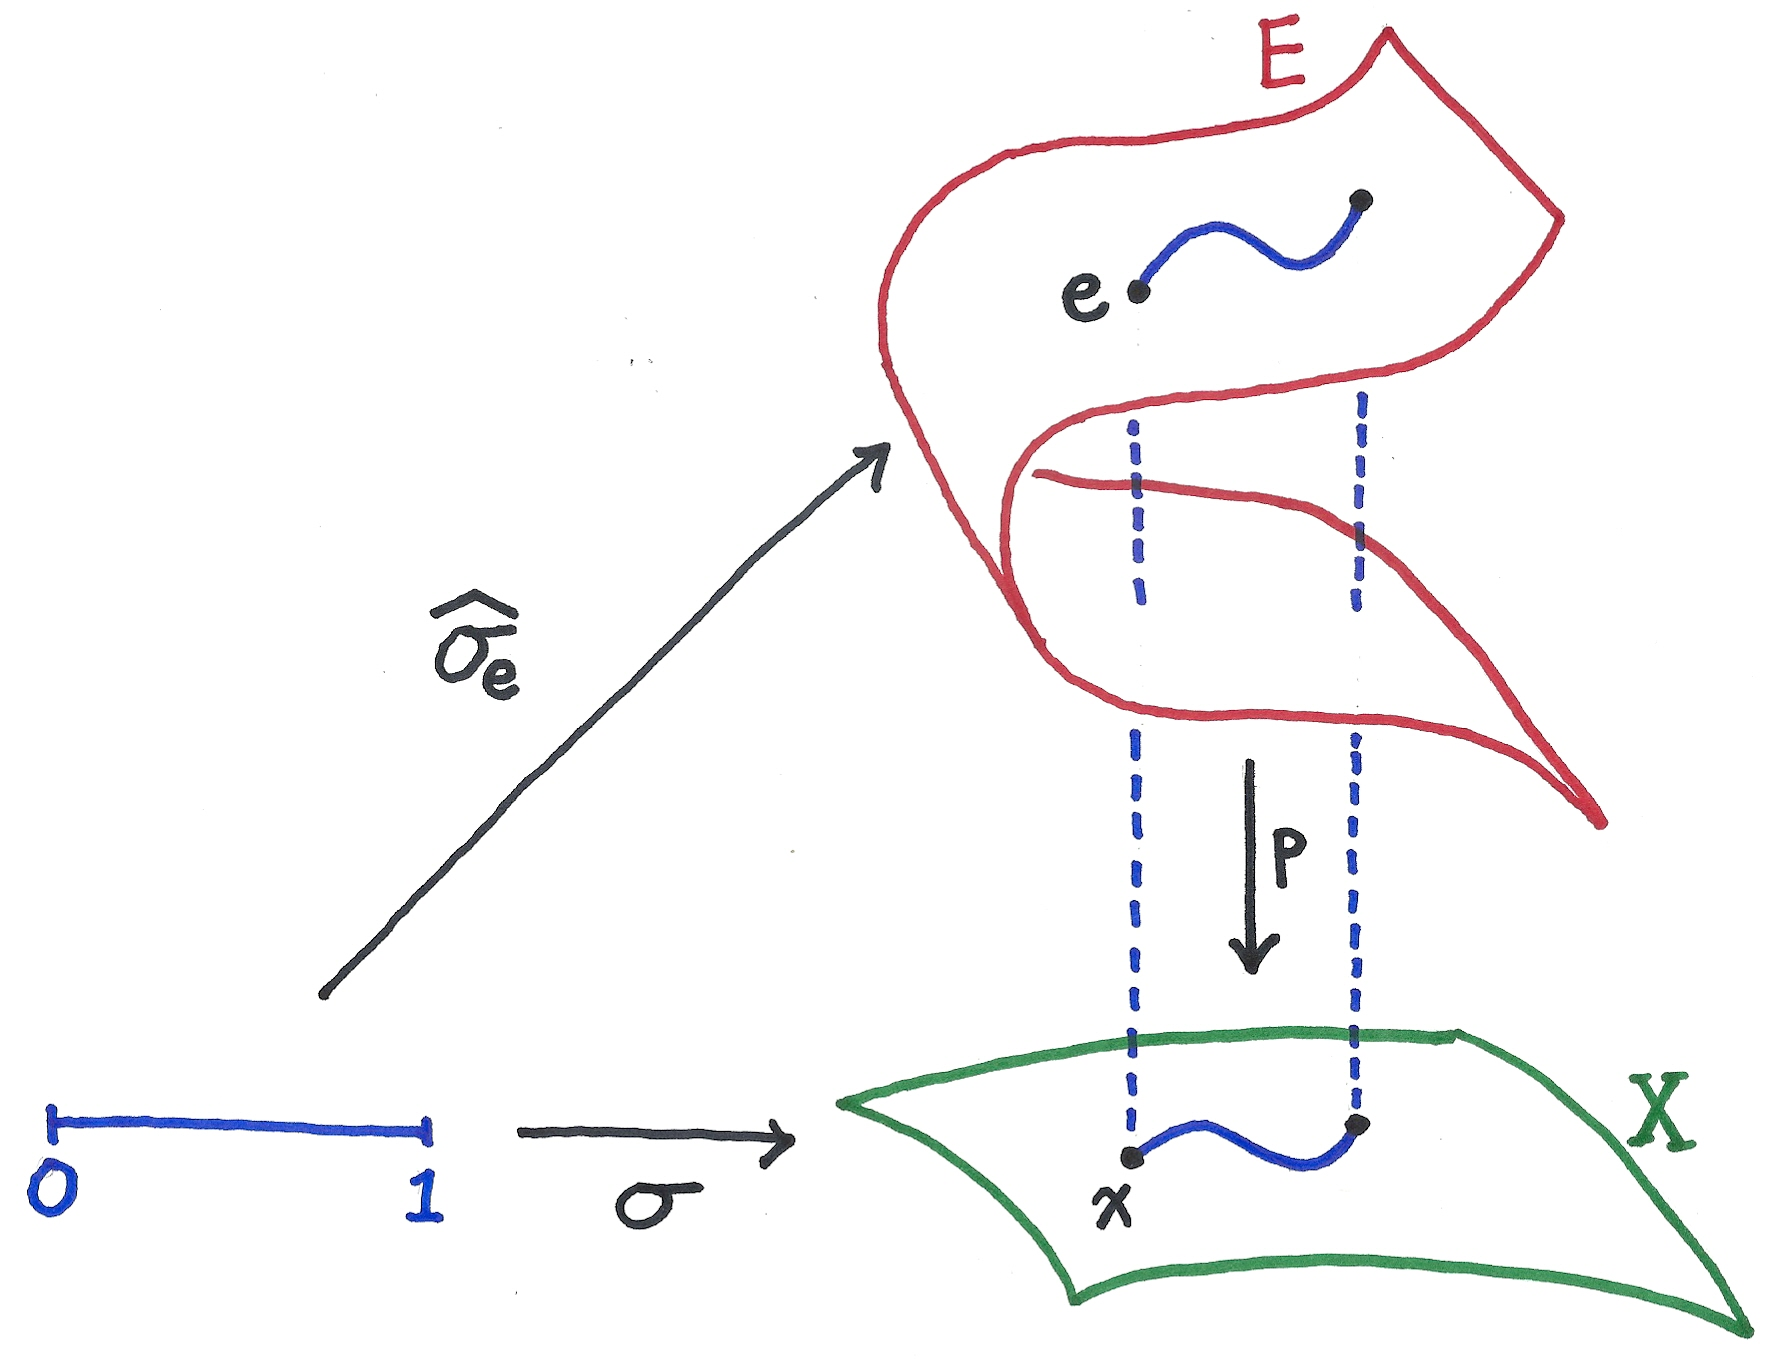
\includegraphics[scale=0.10]{levantamiento}
\end{figure}

\begin{proof}
  Por la definici\'on de cubriente, toda $\sigma(s)\in X$, tiene una vecindad $V_s\subseteq X$
  tal que la restricci\'on de la aplicaci\'on cubriente $p$ a cada componente conexa de
  $p^{-1}[V]$ es un homeomorfismo. Como la imagen de $\sigma$ es compacto, existen
  $0=s_0<s_1<\cdots<s_{n-1}<s_n=1$ tal que $\{V_{s_k}\}_{k=0,\ldots,n}$ es una cubierta de la
  trayectoria. Observa que dos abiertos consecutivos $V_{s_{k-1}}$ y $V_{s_k}$ deben intersectarse
  porque si son disjuntas, $\{V_{s_{k-1}},V_{s_k}\}$ ser\'ia una disconexi\'on de conjunto conexo
  $\sigma[s_{k-1},s_k]$.

  Ahora, si elijo un $e\in E_x$, entonces existe un \'unico componente $U_0$ de $p^{-1}[V_{s_0}]$
  tal que $e\in U_0$. Adem\'as, como $p|_{U_0}:U_0\ra V_{s_0}$ es un homeomorfismo, entonces defino
  \[
    \what{\sigma}_e^0:[0,s_1]\lra V_{s_0}E \quad\text{con}\quad
    \what{\sigma}_e^0(s)=(p|_{U_0})^{-1}(\sigma(s))
  \]
  Observa que $p(\what{\sigma}_e^0(s_1))=\sigma(s_1)\in V_{s_1}$, entonces se determina un
  \'unico componente $U_1$ de $p^{-1}[V_{s_1}]$ tal que $\what{\sigma}_e^0(s_1)\in U_1$. De la
  misma manera, $p|_{U_1}$ es un homeomorfismo y defino
  \[
    \what{\sigma}_e^1:[s_1,s_2]\lra V_{s_1}E \quad\text{con}\quad
    \what{\sigma}_e^1(s)=(p|_{U_1})^{-1}(\sigma(s)).
  \]

  De manera inductiva defino las (\'unicas) $n$ funciones continuas
  $\what{\sigma}_e^k:[s_k,s_{k+1}]\ra U_k$ que coinciden en sus intersecciones. Entonces existe una
  \'unica funci\'on continua $\what{\sigma}_e:I\ra \bigcup U_k\subseteq E$ que se restrinje a cada
  $\what{\sigma}_e^k$.

  Por \'ultimo, para toda $s\in I$, existe una $k$ tal que $s\in[s_k,s_{k+1})$ entonces:
  \[
    (p\circ \widehat{\sigma}_e)(s)=p(\widehat{\sigma}^k_e(s))=p(p|_{U_k})^{-1}(\sigma(s)))=\sigma(s)
  \]
  y la trayectoria $\what{\sigma}_e$ es la buscada.  
\end{proof}

Se puede generalizar el concepto de un cubriente:

\begin{defin}
  Una funci\'on continua $p:E\ra X$ es una \emph{fibraci\'on} si dadas funciones $g,f:Y\ra E$
  y una homotop\'ia  $H:Y\times I\ra X$ entre $p\circ f:Y\ra X$ y $p\circ g: Y\ra X$, existe una
  \'unica homotop\'ia $\what{H}:Y\times I\ra E$ entre $f$ y $g$ que extiende a $H$, es decir
  se tiene el siguiente diagrama conmutativo:
  \[
    \begin{tikzcd}
      Y \arrow[dd,"(\Id\text{,}0)"'] \arrow[rr,"f"] && E \arrow[dd,"p"] \\ &&  \\
      Y\times I \arrow[rr,"H"'] \arrow[uurr,dashed,"\what{H}"] && X
    \end{tikzcd}
    \qquad\quad p\circ\what{H}=H.
  \]
\end{defin}

\begin{thm}\label{thm:cubriente_implica_fibracion}
  Todo cubriente $p:E\ra X$ es una fibraci\'on.
\end{thm}

En el caso del teorema del levantamiento, la elecci\'on de $e\in E$ es equivalente a tomar $Y=\{e\}$.

Ahora me enfoco en usar los cubrientes para calcular los grupos fundamentales:

\begin{prop}
  Sea $p:E\ra X$ un cubriente con $(X,x)$ un espacio basado y $e\in E_x$. Entonces el morfismo
  inducido $(p_{\#}):\pi_n(E,e)\ra\pi_n(X,x)$ es un monomorfismo de grupos para toda $n$.
\end{prop}
\begin{proof}
  Sea $[\alpha]\in\pi_n(E,e)$ (en particular $\alpha:\Sn^n\ra E$) tal que
  $(p_{\#})[\alpha]=[p\circ\alpha]=1$, es decir que
  $p\circ\alpha \simeq \text{cte}_x:\Sn^n\ra\{x\}\subset X$. Sea $H:I\times I\ra E$ tal
  homotop\'ia con $H_0(t)=\text{cte}_x(t)=x$ y $H_1(t)=(p\circ\alpha)(t)$.

  Por el teorema \ref{thm:cubriente_implica_fibracion}, $p:E\ra X$ es una fibraci\'on y si tomo
  $Y=I$ entonces existe una homotop\'ia $\what{H}:I\times I\ra E$ entre $\alpha$ y el lazo
  constante $\cte_e(s)=e\in E$ (que es el que cumple $p\circ \text{cte}_e=\text{\cte}_x$). Por lo tanto
  $(p_{\#})[\alpha]=[p\circ\alpha]=[\text{cte}_e]=1\in\pi_n(E,e)$ y $p_{\#}$ es un monomorfismo.
\end{proof}

Ahora si restrinjo al caso $n>1$ el morfismo $(p_{\#}):\pi_n(E)\ra\pi_n(X,x)$ es un ismorfismo! Esto
sucede porque bajo ciertas condiciones, cualquier funci\'on continua $f:Y\ra X$, en particular $Y=\Sn^n$,
se factoriza a trav\'es del cubriente $p:E \ra X$:

\begin{thm}\label{thm:factoriza_atrd_cubriente}
  Sea $p:E\ra X$ un cubriente visto en $\cat{Top}_*$ con $(E,e)$ y $(X,x)$ tal que $e\in E_x$.
  Si $(Y,y)$ es conexo y localmente conectable por trayectorias y $f:Y\ra X$ es basada, entonces:
  \[
    \begin{tikzcd}
      & E \arrow[d,"p"] \\
      Y \arrow[ur,dashed,"\exists!\what{f}"] \arrow[r,"f"'] & X
    \end{tikzcd} \quad\iff\quad f_{\#}\big[\pi_1(Y) \big] \subseteq p_{\#}\big[\pi_1(E) \big]
  \]
\end{thm}

\import{\directory}{ejercicios/27} %%%%%%%%%%%%%%%%%%%%%%%%%%%%%%%%%%%%%%%%%%%%%%% EJERCICIO 27

\begin{nota}
  Para la ida no se requiri\'o que $Y$ fuese conexa y localmente conectable por trayectorias.
\end{nota}

El regreso de del teorema \ref{thm:factoriza_atrd_cubriente} se hace de la siguiente manera:

Sea $\sigma:I\ra Y$ una trayectoria que empieza en $\sigma(0)=y$ y termina en $\sigma(1)=y'$.
Entonces $f_*(\sigma):=f\circ\sigma:I\ra X$ es una trayectoria y por el teorema del
levantamiento existe una \'unica trayectoria $\what{f_*(\sigma)}_e:I\ra E$ que extiende a
$f_*(\sigma)$. Con esto defino:
\[
  \what{f}:Y \lra E \quad\text{con}\quad \what{f}(y')=\what{f_*(\sigma)}(1)
\]
Ve:
\begin{figure}[ht] %%%%%%%%%%%%%%%%%%%%%%%%%%%%%%%%%%%%%%%%%%%%%%%%%%%%%%%%% FACTORIZA_ATRD_CUBRIENTE
  \centering
  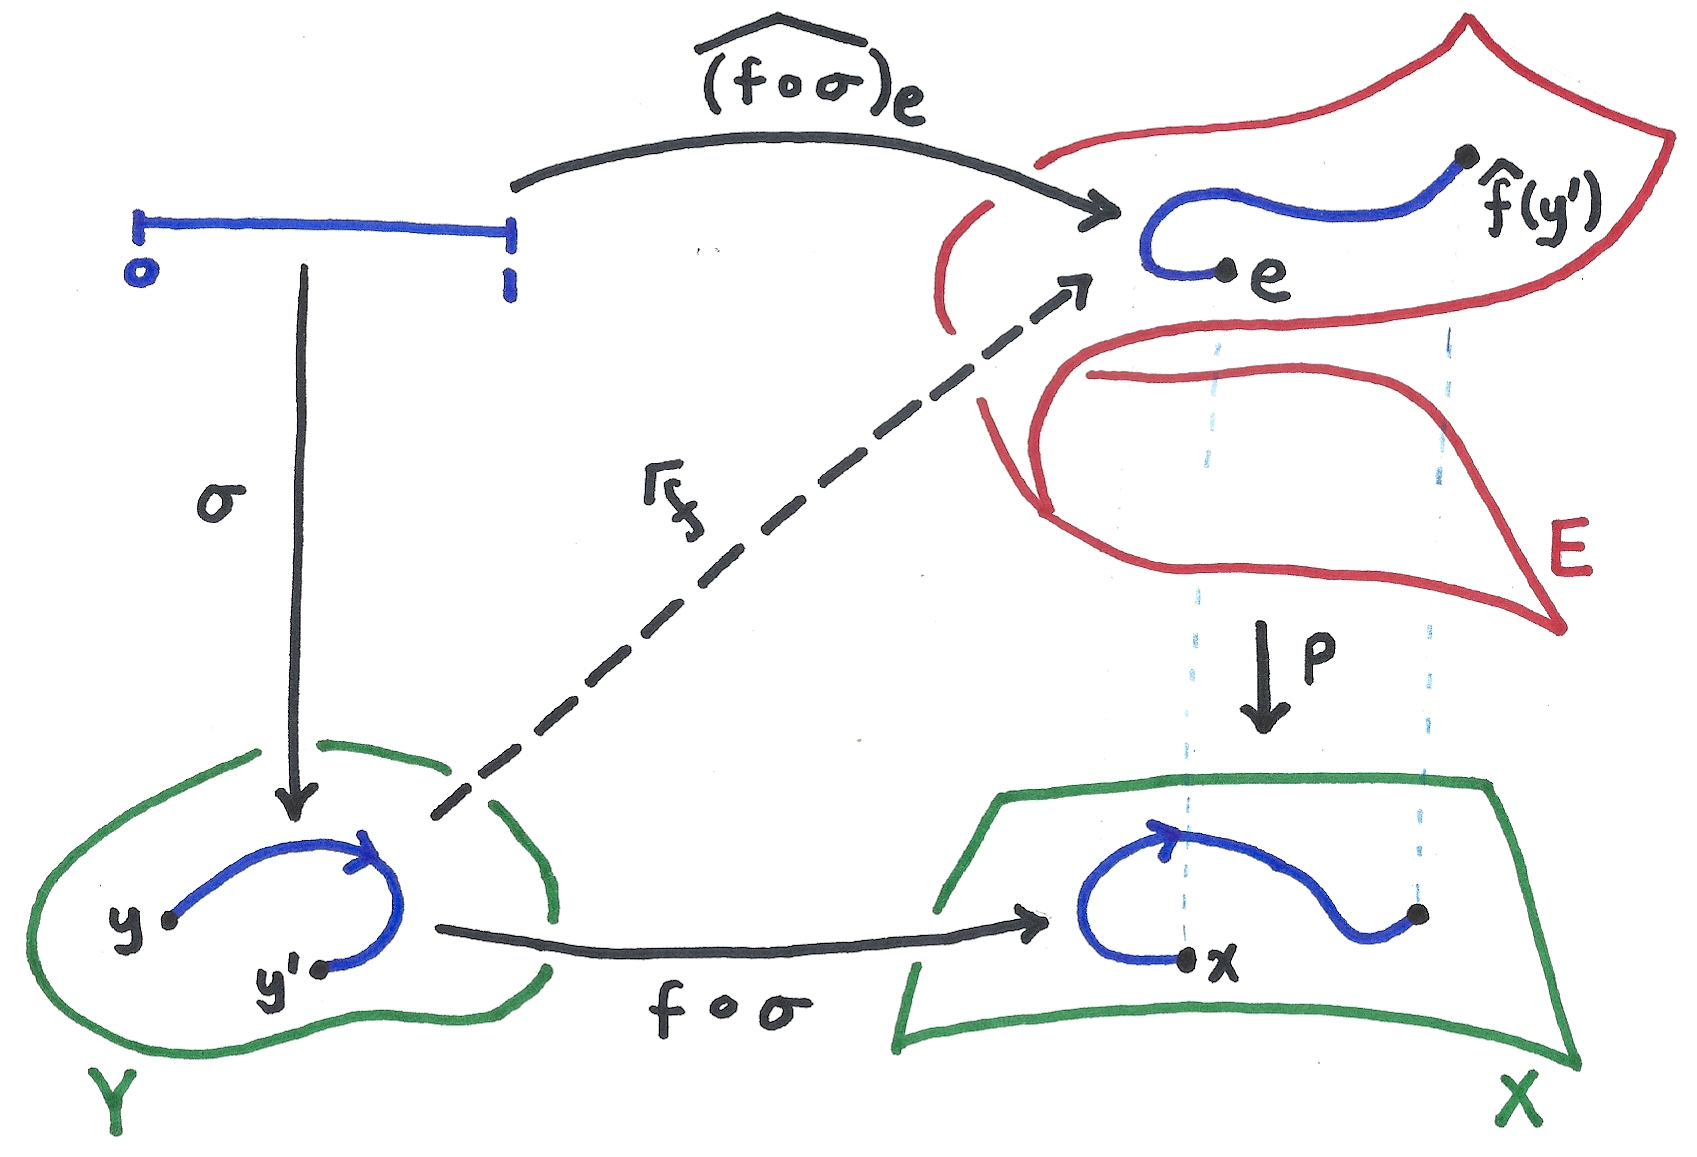
\includegraphics[scale=0.13]{factoriza_atrd_cubriente}
\end{figure}%%%%%%%%%%%%%%%%%%%%%%%%%%%%%%%%%%%%%%%%%%%%%%%%%%%%%%%%%%%%%%%%%%%%%%%%%%%%%%%%%%%%%%%%

Observa que $\what{f}$ est\'a bien definido porque si $\tau:I\ra Y$ es otra trayectoria que empieza
en $y$ y termina en $y'$...........................................................................
...................................................................................................

\begin{cor}
  Sea $p:E\ra X$ un cubriente. Entonces para toda $n>1$, el monomorfismo $p_{\#}:\pi_n(E)\ra\pi_n(Y)$
  es un isomorfismo, en s\'imbolos:
  \[
    p:E\ra X \quad\text{es un cubriente} \quad\then\quad \pi_n(E)\cong\pi_n(X) \quad(n>1).
  \]
  
\end{cor}
\begin{proof}
  Nada m\'s tengo que probar que $p_{\#}$ es sobre. Observa que $\Sn^n$ es conexa y y contectable
  por trayectorias. Adem\'as $\pi_1(\Sn^n)=0$ por la ecuaci\'on (\ref{eq:pi_m<n}) entonces para
  toda $\alpha:\Sn^n\ra X$ tengo $\alpha_{\#}[\pi_1(\Sn^n)]=0\subset p_{\#}[\pi_1(E)]$, por el
  teorema \ref{thm:factoriza_atrd_cubriente} existe un $\what{\alpha}:\Sn^n\ra E$ que extiende
  $\alpha$. Claramente
  \[
    p_{\#}[\what{\alpha}]=[p\circ\what{\alpha}]=[\alpha]
  \]
  y $p_{\#}$ es sobre.
\end{proof}

\begin{ejemplo}
  $\pi_n(\Sn^1)=0$ para toda $n>1$ porque la exponencial $\epsilon:\RR\ra\Sn^1$ es un cubriente
  y $\RR$ es contraible.
\end{ejemplo}

El \'unico grupo de homotop\'ia que falta calcularle a $\Sn^1$ es $\pi_1(\Sn^1)$. Para esto
desarrollo la teor\'ia de acciones de grupos.

\subsection{Acciones de grupos}

En esta parte generalizo las acciones de grupos a espacios topol\'ogicos.

\begin{defin}
  Sea $G$ un grupo topol\'ogico con neutro $1\in G$ y $X$ un espacio topol\'ogico. Una
  \emph{acci\'on izquierda} de $G$ en $X$ es una funci\'on continua $G\times X\ra X$ con
  $(g,x)\mapsto gx$ que cumple dos propiedades:
  \begin{enumerate}
  \item[($i$)] $1 x =x\;$ para toda $x\in X$.
  \item[($ii$)] $(g g') x= g(g' x)\;$ para todas $g,g'\in G$.
  \end{enumerate}
\end{defin}

En general una acci\'on de grupo se define sin topolog\'ias pero este caso es un caso particular
de la definici\'on anterior si $G$ y $X$ tienen la topolog\'ia discreta.

\begin{ejemplo}
  Si $G=\text{GL}_n(\RR)$ y $X=\RR^n$ entonces la multiplicaci\'on de matrices $(A,x)\mapsto Ax$
  es una acci\'on de grupo.
\end{ejemplo}

\import{\directory}{ejercicios/28} %%%%%%%%%%%%%%%%%%%%%%%%%%%%%%%%%%%%%%%%%%%%%%% EJERCICIO 28

\begin{defin}
  Sea $G\times X\ra X$ una acci\'on izquierda de un grupo $G$ y $x\in X$ un elemento arbitrario.
  El \emph{grupo de isotrop\'ia} de $x$ es el conjunto de elementos de $G$ que fijan a $x$ bajo
  la acci\'on, es decir:
  \[
    G_x:=\{g\in G \mid gx=x\}.
  \]
\end{defin}

\import{\directory}{ejercicios/29} %%%%%%%%%%%%%%%%%%%%%%%%%%%%%%%%%%%%%%%%%%%%%%%% EJERCICIO 29

\begin{defin}
  Sea $G\times X\ra X$ una acci\'on izquierda de un grupo $G$ y $x\in X$ un elemento arbitrario.
  La \emph{\'orbita} de $x$ es el subconjunto de $X$ definido por
  \[
    \Oo(x):=\{gx\in X\mid g\in G\}.
  \]
\end{defin}

Resulta que las \'orbitas de una acci\'on de grupos sobre $X$ particionan a $X$:

\import{\directory}{ejercicios/30} %%%%%%%%%%%%%%%%%%%%%%%%%%%%%%%%%%%%%%%%%%%%%%%%%%%% EJERCICIO 30

\begin{defin}
  Sea $G\times X\ra X$ una acci\'on de grupos entonces el espacio de cocientes m\'odulo la
  relaci\'on de equivalencia $x\sim y\iff y\in\Oo(x)$ se llama el \emph{espacio de \'orbitas}
  y viene equipada de la topolog\'ia cociente; se denota por $X/G$.
\end{defin}

\begin{nota}
  Las fibras de la identificaci\'on $\nu:X \epi X/G$ son las \'orbitas $\nu^{-1}[x]=\Oo(x)$. 
\end{nota}

Para calcular las \'orbitas de una acci\'on $G\times X\ra X$ restrinjo la acci\'on a
$G\times\{x\}\ra X$, entonces la imagen es exactamente la \'orbita de $x$. Como
$G\approx G\times\{x\}$,  la restricci\'on de la acci\'on se puede ver como la funci\'on continua:
\[
  \a_x:G \lra \Oo(x) \quad ,\quad \a_x(g)=gx.
\]

Adem\'as $\a_x(g)=\a_x(h)\iff gx=hx \iff gh^{-1}\in G_x$. Por lo tanto se factoriza a trav\'es de
la identificaci\'on $\nu:G\epi G/G_x$. Por lo tanto el siguiente diagrama conmuta:
\[
  \begin{tikzcd}
    G \arrow[d,two heads,"\nu"'] \arrow[r,"\a_x"] & \Oo(x) \\
    \tfrac{G}{G_x} \arrow[ur,dashed,"\bar{\a}_x"']
  \end{tikzcd} \quad
  \a_x=\bar{\a}_x\circ\nu.
\]
Est\'a definida por $\a_x(gG_x)=\a_x(g)=gx$. Como $\a_x$ es continua, $\bar{\a}_x$ es continua.
Claramente es sobreyectiva porque $\Oo(x)$ es por definici\'on la imagen de $\a_x$. Adem\'as:

\import{\directory}{ejercicios/31}%%%%%%%%%%%%%%%%%%%%%%%%%%%%%%%%%%%%%%%%%%%%%%%%%%%% EJERCICIO 31

\begin{nota}
  Si $X$ es Hausdorff y $G$ es compacto (y por lo tanto tambi\'en $G/G_x$), entonces por el
  resultado anterior $\bar{\a_x}$ es un homeomorfismo, ie $(G/G_x)\approx\Oo(x)$.
\end{nota}

\begin{defin}
  Una acci\'on $G\times X\ra X$ de grupos es \emph{libre} si $gx=x \then g=1$ o equivalentemente
  $G_x=1$. Es \emph{transitiva} si para cualesquiera $x,y\in X$ existe un $g\in G$ tal que
  $xg=y$ o equivalentemente $X=\Oo(x)$.
\end{defin}

Si $G\times X\ra X$ es una acci\'on libre, la nota anterior dice que si $G$ es compacto y
$X$ hausdorff, entonces $G\approx\Oo(x)$ Observa que este homeomorfismo depende de que $x\in X$
eligimos. Por lo tanto $\Oo(x)$ no hereda una estructura de grupo topol\'ogico. Pero las fibras
de la identificaci\'on $X\epi X/G$ son $\Oo(x)\approx G$. Por lo tanto si $G$ tiene la topolog\'ia
discreta, entonces $\nu:X\ra X/G$ es casi un cubriente; necesitamos que las fibras se vean as\'i
localmente.

\begin{defin}
  Sea $G$ un grupo discreto. Una acci\'on $G\times X\ra X$ es \emph{propiamente discontinua}
  si para toda $x\in X$ tiene una vecindad abierta $U\subseteq X$ tal que
  \[
    gU \cap U = \emptyset \qquad \forall g\neq 1
  \]
  donde $gU$ es la imagen de la restricci\'on de la acci\'on a $G\times U$.
\end{defin}

\import{\directory}{ejercicios/32}%%%%%%%%%%%%%%%%%%%%%%%%%%%%%%%%%%%%%%%%%%%%%%%%% EJERCICIO 32

La importancia de acciones propiamente discontinuas lo muestra el siguiente teorema:

\begin{thm}
  La identificaci\'on $X\ra X/G$ es un cubriente cuando la acci\'on es propiamente discontinua:
  \[
    G\times X\ra X\;\;\text{es propiamente discontinua} \quad\then\quad
    \nu:X\lra X/G \;\;\text{es un cubriente}.
  \]
\end{thm}

\begin{ejemplo}\label{ej:z2_actua_sobre_sn}
  Considera la acci\'on de $G=\ZZ_2$ sobre $X=\Sn^n$ definida como $(\pm 1,x)\mapsto \pm x$.
  Esta acci\'on es libre porque en $\Sn^n$, siempre se cumple que $-x\neq x$. Adem\'as, $\Sn^n$
  es Hausdorff y $G$ es compacto (por ser finito y discreto), entonces el teorema anterior aplica:
  \[
    \Sn^n \lra \Sn^n/Z_2 = \RR P^2 \quad\text{es un cubriente}.
  \]
\end{ejemplo}

Los espacios cubrientes nos permiten estudiar los grupos fundamentales porque para todo cubriente
existe una acci\'on de grupo especial:

\begin{defin}
  Sean $p:E\ra X$ un cubriente, $x\in X$ fijo y $E_x$ la fibra de $p$ sobre $x$. El grupo
  fundamental $\pi_1(X,x)$ act\'ua  sobre la fibra $E_x$ de la siguiente manera:
  \[
    E_x \times \pi_1(X) \lra E_x \quad ,\quad (e,[\sigma]) \mapsto \what{\sigma}_e(1)
  \]
  donde $\what{\sigma}_e:I\ra E$ es el levantamiento de $\sigma$ a $E$ garantizado por el
  teorema \ref{thm:levantamiento}.
\end{defin}

%\begin{figure}[ht]
%  \centering
%  \includegraphics[scale=1.2]{accion_grupo_fundamental}
%\end{figure}

\import{\directory}{ejercicios/33} %%%%%%%%%%%%%%%%%%%%%%%%%%%%%%%%%%%%%%%%%%%%%%%% EJERCICIO 33

\import{\directory}{ejercicios/34} %%%%%%%%%%%%%%%%%%%%%%%%%%%%%%%%%%%%%%%%%%%%%%%% EJERCICIO 34

Si aplico estos dos resultados al ejemplo \ref{ej:z2_actua_sobre_sn} puedo calcular el grupo
fundamental del espacio proyectivo:

\begin{prop}
  Para toda $n>1$, $\pi_1(\RR P^n)\cong \ZZ_2$.
\end{prop}
\begin{proof}
  Por el ejemplo \ref{ej:z2_actua_sobre_sn}, la identificaci\'on $p:\Sn^n\ra\RR P^n$ es un
  cubriente inducido por la acci\'on de $\ZZ_2$ sobre $\Sn^n$. Si escribo $G=\pi_1(\RR P^n)$
  entonces $G$ act\'ua sobre las fibras $E_{[x]}=\{x,-x\}$.

  Por el ejercicio \ref{ej:33},
  como $\Sn^n$ es conectable por trayectorias, esta acci\'on es transitiva y as\'i
  $\Oo([x])=E_{[x]}$. El ejercicio \ref{ej:31} garantiza que $G/G_e$ y $E_{[x]}$ est\'an en
  biyecci\'on, es decir el grupo $G/G_e$ tiene dos elementos; por lo tanto es isomorfo a $\ZZ_2$.
  Por \'ultimo, el ejercicio \ref{ej:34} dice que $G_e=p_{\#}[\pi_1(\Sn^n)]=p_{\#}[1]=1$ (donde
  $\pi_1(\Sn^n)=1$ por la f\'ormula \ref{eq:pi_m<n}) entonces $G/G_e\cong G$ y concluyo que
  $\pi_1(\RR P^n)=\ZZ_2$.  
\end{proof}

Ya tengo la herramienta necesaria para poder calcular el \'ultimo grupo fundamental de $\Sn^1$ que
falta calcular:

Por el ejercicio \ref{ej:26}, la exponencial $\epsilon:\RR\ra\Sn^1$ es un cubriente, entonces
hay acci\'on $\a$ sobre la fibra $\RR_1=\epsilon^{-1}(1)=\ZZ$ asociada al cubriente. Adem\'as esta
acci\'on es transitiva por el ejercicio \ref{ej:33} y as\'i $\Oo(n)=\ZZ$ para toda $n\in\ZZ$.
  
Si escribo $G=\pi_1(\Sn^1,1)$ entonces $\a_n:G\ra\Oo(n)=\ZZ$, induce una biyecci\'on continua
$\bar{\a}_n:(G/G_n)\ra\ZZ$. Observa que $\RR$ es contraible, entonces el ejercicio \ref{ej:24}
garantiza que $G_n=\epsilon_{\#}[\pi_1(\RR,0)]=\epsilon_{\#}[1]=1$. Por lo tanto $G\cong G/G_n$
y $\bar{\a}_n:G\ra\ZZ$ es una biyecci\'on continua para toda $n$. En general $\bar{\a}_n$ est\'a
definido por $\bar{\a}_n[\sigma]=n[\sigma]=\what{\sigma}_n(1)$. Resulta que:

\import{\directory}{ejercicios/35} %%%%%%%%%%%%%%%%%%%%%%%%%%%%%%%%%%%%%%%%%%%%%%%%%%%% EJERCICIO 35

Por lo tanto he demostrado que

\begin{prop}
  $\pi_1(\Sn^1,1)\cong\ZZ$.
\end{prop}

Los cubrientes forman una categor\'ia:

\begin{defin}
  Sea $X$ un espacio topol\'ogico fijo. La categor\'ia de cubrientes sobre $X$, denotado por
  $\cat{Cub}(X)$, tiene como objetos los cubrientes $(E,p,X)$ y morfismos las funciones
  continuas $f:(E,p,X)\ra(E',p',X)$ que hacen conmutar el siguiente diagrama:
  \[
    \begin{tikzcd}
      E \arrow[rr,"f"] \arrow[dr,"p"'] && E' \arrow[dl,"p'"] \\
      & X &
    \end{tikzcd}
  \]
\end{defin}

\begin{thm}
  Sea $X$ un espacio conexo, localmente conectable por trayectorias y semilocalmente 1-conexo
  (alrededor de cada punto existe una vecindad $U\subseteq X$ cuya inclusi\'on $\imath:U\ra X$
  induce el morfismo cero, es decir $\imath_{\#}=0$). Existe una biyecci\'on
  \[
    \cat{Cub}(X) \longleftrightarrow \{H\leq\pi_1(X)\}/_{gHg^{-1}}
  \]
\end{thm}

\begin{ejemplo}
  Si $n>1$, $\cat{Cub}(\Sn^n)=\{\Id\}$ porque $\pi_1(\Sn^n)=0$.
\end{ejemplo}


\end{document}
